\chapter{IMPLEMENTATION AND TESTS}
First of all, in this project only several syntax and statement models are implemented in the given time. That's why, the tests and experiments are limited.

In the test file, there are some integer overflows, an array bound overflow (which occurs when trying to access outside of an allocated area) and a stack-heap based overflow which occurs in a vulnerable C library function strcpy(). Figure \ref{fig:TestCode} shows the test code.

\begin{figure}[!htbp]
    \centering
    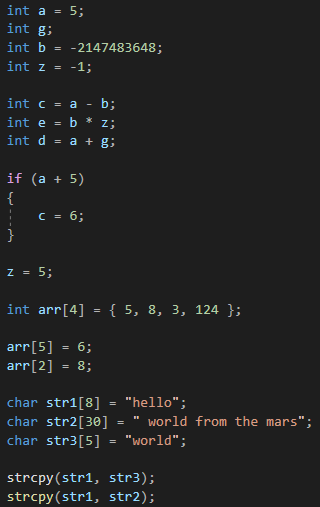
\includegraphics[width=0.4\textwidth]{Imgs/test_code2.png}
    \caption{\label{fig:TestCode} The test file}
\end{figure}

In figure \ref{fig:TestResult}, the overflow analysis of our program showed in graphical user interface.

In figure \ref{fig:TestResult}, the overflow analysis results of our program are showed in a user interface.

\clearpage

\begin{figure}[!htbp]
    \centering
    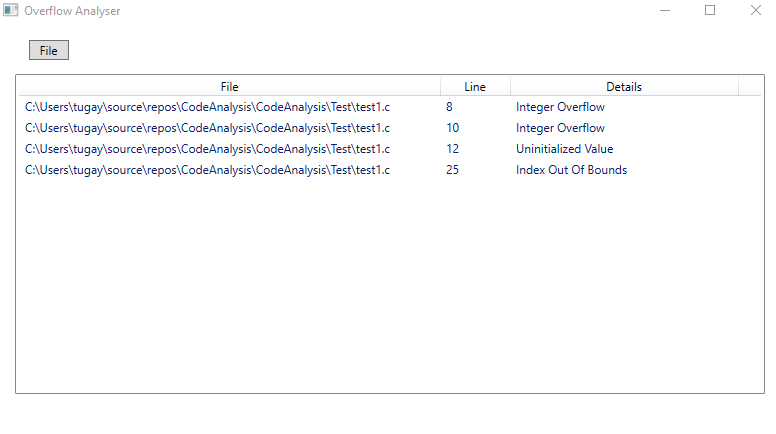
\includegraphics[width=0.7\textwidth]{Imgs/test_result.png}
    \caption{\label{fig:TestResult} An example result list from the GUI}
\end{figure}

In figure \ref{fig:TestCppResult} the same test file is analysed with CppCheck program. It can be seen that the only difference is the overflow that occurs in strcpy() function. 

\begin{figure}[!htbp]
    \centering
    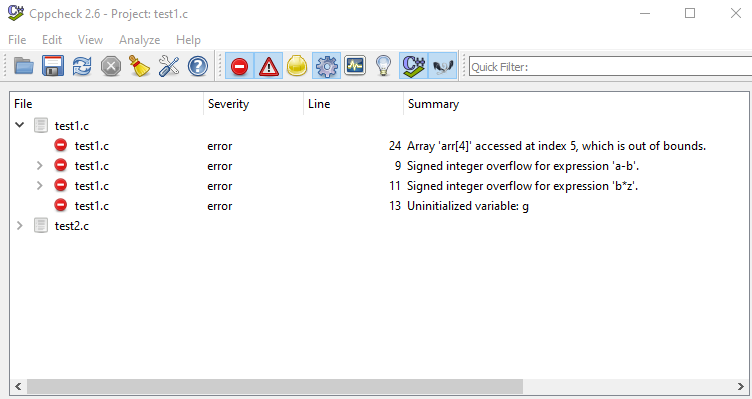
\includegraphics[width=0.8\textwidth]{Imgs/cppcheck_test.png}
    \caption{\label{fig:TestCppResult} CppCheck Results}
\end{figure}

There are many vulnerable C library functions that can cause overflows. But, static analysis can only be done on source code. That's why, static analysis has some disadvantages. In this condition, I manually defined vulnerable C library functions. That's why, my program was able to detect overflow caused at strcpy() function call.